\documentclass[tikz, border=2pt]{standalone}

\usepackage{amsmath,amssymb}
\usepackage{pgfplots}
\pgfplotsset{compat=1.18}
\usepgfplotslibrary{groupplots}
\usetikzlibrary{arrows.meta}
\usepackage{xcolor}

\definecolor{utnblue}{RGB}{0, 51, 102}
\definecolor{utnred}{RGB}{204, 0, 0}

\begin{document}
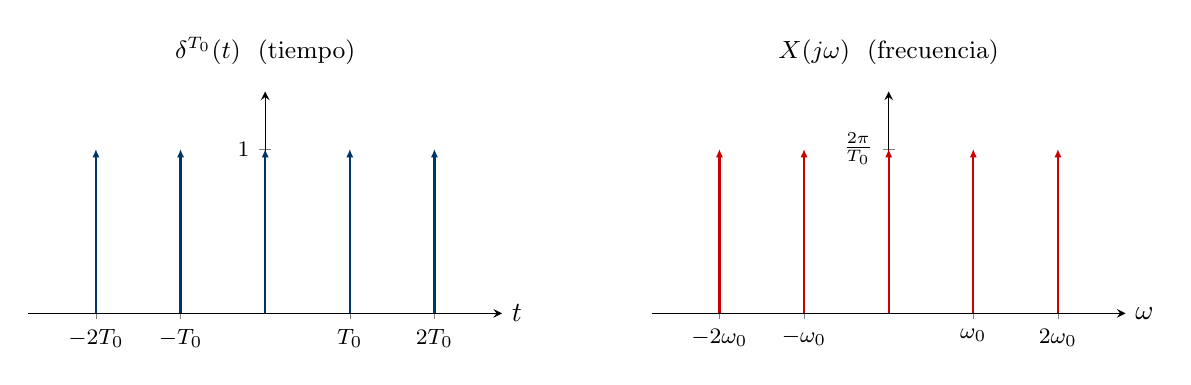
\begin{tikzpicture}[
    impa/.style={utnblue, line width=0.8pt, -{Latex[length=3pt,width=2.6pt]}},
    impf/.style={utnred, line width=0.8pt, -{Latex[length=3pt,width=2.6pt]}},
  ]

\begin{groupplot}[
    group style={group size=2 by 1, horizontal sep=1.9cm},
    width=7.6cm, height=4.4cm,
    axis lines=middle,
    enlargelimits=false,
    tick label style={font=\footnotesize},
    label style={font=\small},
    title style={font=\small},
    every axis x label/.style={at={(ticklabel* cs:1)}, anchor=west},
]

% --- Panel: tren en el tiempo ---
\nextgroupplot[
    title={$\delta^{T_0}(t)$ \ (tiempo)},
    xlabel={$t$},
    xmin=-2.8, xmax=2.8, ymin=0, ymax=1.35,
    xtick={-2,-1,1,2}, xticklabels={$-2T_0$,$-T_0$,$T_0$,$2T_0$},
    ytick={1}, yticklabels={$1$},
]
\draw[impa] (axis cs:-2,0) -- (axis cs:-2,1);
\draw[impa] (axis cs:-1,0) -- (axis cs:-1,1);
\draw[impa] (axis cs: 0,0) -- (axis cs: 0,1);
\draw[impa] (axis cs: 1,0) -- (axis cs: 1,1);
\draw[impa] (axis cs: 2,0) -- (axis cs: 2,1);

% --- Panel: tren en frecuencia ---
\nextgroupplot[
    title={$X(j\omega)$ \ (frecuencia)},
    xlabel={$\omega$},
    xmin=-2.8, xmax=2.8, ymin=0, ymax=1.35,
    xtick={-2,-1,1,2}, xticklabels={$-2\omega_0$,$-\omega_0$,$\omega_0$,$2\omega_0$},
    ytick={1}, yticklabels={$\tfrac{2\pi}{T_0}$},
]
\draw[impf] (axis cs:-2,0) -- (axis cs:-2,1);
\draw[impf] (axis cs:-1,0) -- (axis cs:-1,1);
\draw[impf] (axis cs: 0,0) -- (axis cs: 0,1);
\draw[impf] (axis cs: 1,0) -- (axis cs: 1,1);
\draw[impf] (axis cs: 2,0) -- (axis cs: 2,1);

\end{groupplot}

\end{tikzpicture}
\end{document}
